%% implemen.tex
%% $Id: implemen.tex 61 2012-05-03 13:58:03Z bless $
%%

\chapter{Implementierung}
\label{ch:Implementierung}
%% ==============================



\section{iRRAM}
\label{sec:irram}
Die Software-Bibliothek \verb+iRRAM+ \cite{Mller2009EnhancingIE} basiert auf Intervallen als Zahlentyp, um diese mit einer beliebigen Genauigkeit darstellen zu können. Zunächst wird mit Double-Präzision, also 64-Bit Zahlen gerechnet, welche verwendet werden, bis das Ergebnis für die angefragte Präzision nicht mehr genau ausgegeben werden kann, beziehungsweise bis zu einer bestimmten Anzahl an Bits. Ist dies der Fall, geschieht eine Iteration mit einer erhöhten Genauigkeit, also längeren Zahlen, welche dann mit Hilfe von \verb+MPFR+ dargestellt werden.
Für eine solche Iteration werden gerade so viele Zwischenergebnisse während der Berechnung gespeichert, dass eine Wiederholung der Schritte mit höherer Präzision möglich ist. Da nicht die gesamte Berechnung in jeder Iteration wiederholt wird, müssen während der Laufzeit Sichtbarkeit von Variablen und Zwischenergebnissen für den Nutzer genau kontrolliert und unter Umständen beschränkt werden, da sonst unerwartetes Verhalten und Exceptions entstehen können, indem die zugegriffenen Werte gegebenfalls nicht in der aktuellen Iteration existieren.


Einige der für rationale Zahlen zur Verfügung stehenden Funktionen, wie der Vergleich zweier Zahlen, sind mit reellen Zahlen nicht ohne weiteres Möglich. Dies gilt insbesondere für den Test auf Gleichheit und die Vorzeichenfunktion $sign$. Bei all diesen Funktionen handelt es sich im Reellen (und bei der \verb+iRRAM+) um mehrwertige Funktionen, da sich das jeweilige Ergebnis mit veränderter Präzsion in der Darstellung der Zahlen ändern kann. Dieses Problem wird in \verb+hotm+ durch den \verb+SignType+ adressiert. Zusätzlich zu den Werten 'positiv' (=\verb+POS+) und 'negativ' (=\verb+NEG+),  kann die Vorzeichenfunktion \verb+sign+ den Wert 'ambivalent' (=\verb+AMBI+) ausgeben, wenn nicht entscheidbar ist, wo genau die reelle Zahl um die Null liegt. Hierfür erhält die Vorzeichenfunktion einen Parameter, der den Bereich er Unsicherheit definiert. Ist der Ausgabewert 'ambivalent', so wird in den Funktionen, welche die Vorzeichenfunktion aufrufen, der schlechteste Fall im Hinblick auf die Genauigkeit, beziehungsweise die Intervallbreite des Ergebnisses angenommen. 


Eine weitere Besonderheit ergibt sich aus dem Aufbau der Zahlen. Es entstehen zwei Intervall-`Ebenen`: Zum Einen, die Darstellung des Koeffizienten als Intervall aus Mitte und Radius. Zum Anderen die Darstellung von Mitte und Radius, als \verb+iRRAM-REAL+, also auch wiederum jeweils als Intervall mit Wert und Fehler, wie in Grafik \ref{fig:levels} zu sehen ist. Im Vergleich zu den \verb+mpq-RATIONALS+ erhöht sich hier zwar die Komplexität deutlich, allerdings lassen sich Ungenauigkeiten sehr genau steuern, indem zum Beispiel der Rechenfehler des Mittelpunkts eines Koeffizienten auf den Radius 'verlagert' wird. So vergrößert sich zwar der Radius des Koeffizienten, welcher dadurch ungenauer wird, jedoch verkleinert sich der Rechenfehler auf der Zahlenebene der \verb+REAL+s. Ein ählicher Effekt sollte sich durch Rundung auch mit den \verb+mpq-RATIONALS+ erreichen lassen. 


Das Verlagern der Ungenauigkeit ($e$ in der Grafik \ref{fig:levels}) auf den Wert des Radius' ($v$ in der Grafik) (Cleaning oder auch \textit{Micro-Housekeeping}) verringert die Intervallbreite und erzeugt Punktintervalle auf der Zahlenebene, allerdings werden die Intervalle auf der Intervallebene breiter. Hier greift dann wiederum der Polish-Mechanismus, der auf Polynomebene Monome hinzufügt, um aus den zu groß gewordenen Intervallen wiederum Punktintervalle zu machen (Splitting oder auch \textit{Macro-Housekeeping}). So wird der Rechenfehler von der untersten Ebene bis zur Polynomebene propagiert.
Diese Housekeeping-Funktionen werden durch Parameter gesteuert, die bestimmen, ab wann ein Intervall zu breit ist und die jeweilige Prozedur angewandt werden soll.




\begin{figure}[tbh]
\begin{center}
 
 

\tikzset{every picture/.style={line width=0.75pt}} %set default line width to 0.75pt        

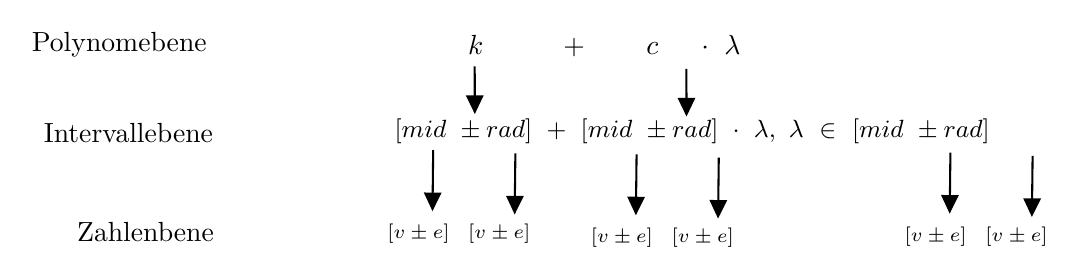
\begin{tikzpicture}[x=0.75pt,y=0.75pt,yscale=-1,xscale=1]
%uncomment if require: \path (0,300); %set diagram left start at 0, and has height of 300

%Straight Lines [id:da29898159624783616] 
\draw    (281.07,90.5) -- (280.77,116.88) ;
\draw [shift={(280.73,119.88)}, rotate = 270.65] [fill={rgb, 255:red, 0; green, 0; blue, 0 }  ][line width=0.08]  [draw opacity=0] (8.93,-4.29) -- (0,0) -- (8.93,4.29) -- cycle    ;
%Straight Lines [id:da1335093356184387] 
\draw    (320.67,92.1) -- (320.37,118.48) ;
\draw [shift={(320.33,121.48)}, rotate = 270.65] [fill={rgb, 255:red, 0; green, 0; blue, 0 }  ][line width=0.08]  [draw opacity=0] (8.93,-4.29) -- (0,0) -- (8.93,4.29) -- cycle    ;
%Straight Lines [id:da1340726243132735] 
\draw    (379.07,92.5) -- (378.77,118.88) ;
\draw [shift={(378.73,121.88)}, rotate = 270.65] [fill={rgb, 255:red, 0; green, 0; blue, 0 }  ][line width=0.08]  [draw opacity=0] (8.93,-4.29) -- (0,0) -- (8.93,4.29) -- cycle    ;
%Straight Lines [id:da9182990047680641] 
\draw    (418.67,94.1) -- (418.37,120.48) ;
\draw [shift={(418.33,123.48)}, rotate = 270.65] [fill={rgb, 255:red, 0; green, 0; blue, 0 }  ][line width=0.08]  [draw opacity=0] (8.93,-4.29) -- (0,0) -- (8.93,4.29) -- cycle    ;
%Straight Lines [id:da04610901450657834] 
\draw    (530.27,91.7) -- (529.97,118.08) ;
\draw [shift={(529.93,121.08)}, rotate = 270.65] [fill={rgb, 255:red, 0; green, 0; blue, 0 }  ][line width=0.08]  [draw opacity=0] (8.93,-4.29) -- (0,0) -- (8.93,4.29) -- cycle    ;
%Straight Lines [id:da7044032296577734] 
\draw    (569.87,93.3) -- (569.57,119.68) ;
\draw [shift={(569.53,122.68)}, rotate = 270.65] [fill={rgb, 255:red, 0; green, 0; blue, 0 }  ][line width=0.08]  [draw opacity=0] (8.93,-4.29) -- (0,0) -- (8.93,4.29) -- cycle    ;
%Straight Lines [id:da7628093943540135] 
\draw    (301.07,50.1) -- (301.12,70.08) ;
\draw [shift={(301.13,73.08)}, rotate = 269.84000000000003] [fill={rgb, 255:red, 0; green, 0; blue, 0 }  ][line width=0.08]  [draw opacity=0] (8.93,-4.29) -- (0,0) -- (8.93,4.29) -- cycle    ;
%Straight Lines [id:da9018979196177348] 
\draw    (403.07,51.3) -- (403.12,71.28) ;
\draw [shift={(403.13,74.28)}, rotate = 269.84000000000003] [fill={rgb, 255:red, 0; green, 0; blue, 0 }  ][line width=0.08]  [draw opacity=0] (8.93,-4.29) -- (0,0) -- (8.93,4.29) -- cycle    ;

% Text Node
\draw (86.2,32) node [anchor=north west][inner sep=0.75pt]   [align=left] {Polynomebene};
% Text Node
\draw (92,76) node [anchor=north west][inner sep=0.75pt]   [align=left] {Intervallebene};
% Text Node
\draw (108,124) node [anchor=north west][inner sep=0.75pt]   [align=left] {Zahlenbene};
% Text Node
\draw (296.4,33.8) node [anchor=north west][inner sep=0.75pt]    {$k\ \ \ \ \ \ \ \ +\ \ \ \ \ \  c\ \ \ \ \cdot \ \lambda $};
% Text Node
\draw (261,74) node [anchor=north west][inner sep=0.75pt]  [font=\small]  {$\left[\text{mid} \ \pm \text{rad}\right] \ +\ \left[\text{mid} \ \pm \text{rad}\right] \ \cdot \ \lambda ,\ \lambda \ \in \ \left[\text{mid} \ \pm \text{rad}\right]$};
% Text Node
\draw (257.5,124.6) node [anchor=north west][inner sep=0.75pt]  [font=\scriptsize]  {$\left[\text{v} \pm \text{e}\right] \ \ \left[\text{v} \pm \text{e}\right]$};
% Text Node
\draw (355.5,126.6) node [anchor=north west][inner sep=0.75pt]  [font=\scriptsize]  {$\left[\text{v} \pm \text{e}\right] \ \ \left[\text{v} \pm \text{e}\right]$};
% Text Node
\draw (506.7,125.8) node [anchor=north west][inner sep=0.75pt]  [font=\scriptsize]  {$\left[\text{v} \pm \text{e}\right] \ \ \left[\text{v} \pm \text{e}\right]$};


\end{tikzpicture}
  
 \caption{Ebenen der Polynomdarstellung mit REALs}
 \label{fig:levels}
 \end{center}
\end{figure}


\subsection{Präzision}
Werden zwei \verb+iRRAM-REAL+s $x$ und $y$ mit einer jeweiligen Präzision $p_x$ und $p_y$ verrechnet $z = x \circ y$, so entscheidet die Präzisions-Strategie \verb+prec_policy+, ob für für diese Operation absolute oder relative Genauigkeit verwendet wird. Zudem existiert eine globale, an die Iteration der \verb+iRRAM+ gebundene Genauigkeit \verb+actual_precision+ $p_g$ , die sich mit jeder Iteration verringert, beginnend mit dem Wert $p_{g0} = -50$. Diese Werte sind negativ und repräsentieren, die Anzahl an Bits, für die eine Zahl genau bekannt ist. Bei $z = x\circ y$ ist die Genauigkeit $p_z$ durch
$$p_z = \begin{cases}
         max(p_x, p_y, p_g) & \text{falls absolute Genauigkeit}\\
         max(p_x, p_y, max(p_x, p_y) - 50 + p_g) & \text{falls relative Genauigkeit}
        \end{cases}
$$
gegeben.
Für die Anwendung in \verb+hotm+ eignet sich die Verwendung von relativer Genauigkeit am besten, da die Manipulation der Fehlerbreite durch Cleaning große Unterschiede in der Genauigkeit zwischen Zahlen ergibt und die Skalierung zu auffwändig ist.



\section{Intervallarithmetik}
\label{sec:numint}
Arithmetik auf Taylormodellen zu betreiben bedeutet auf der untersten Ebene, mit Intervallen zu rechnen. Um diese wiederum als Zahlentyp zu verwenden, müssen die Operationen angepasst werden \cite{moore1979}.

\paragraph{Grundrechenarten}
\begin{itemize}
    \item[] $[x_1, x_2] + [y_1, y_2] = [x_1 + y_1, x_2 + y_2]$
    \item[] $[x_1, x_2] - [y_1, y_2] = [x_1 - y_2, x_2 - y_1]$
    \item[] $[x_1, x_2] \cdot [y_1, y_2] = [min(x_1 y_1, x_1 y_2, x_2 y_1, x_2 y_2), max(x_1 y_1, x_1 y_2, x_2 y_1, x_2 y_2)]$
    \item[] $[x_1, x_2] / [y_1, y_2] = [min(x_1 / y_1, x_1 / y_2, x_2 / y_1, x_2 / y_2),$\\ $max(x_1 /y_1, x_1 /y_2, x_2 /y_1, x_2 /y_2)]$
\end{itemize}
\paragraph{Potenzfunktion}\label{par:potenzfunktion}
Die Potenzfunktion unterscheidet zwischen geradem und ungeradem Exponenten.
$$[x_1, x_2]^n =
 \begin{cases}
    [x_1^n, x_2^n] & falls\ x_1 > 0\ oder\ n\ ungerade; \\
    [x_2^n, x_1^n] & falls\ x_2 < 0\ und\ n\ gerade, \\
    [0, max(x_1^n, x_2^n)] & falls\ 0\in [x_1, x_2] \ und\ n\ gerade;
 \end{cases}$$

\paragraph{Kehrwert}
Der Kehrwert eines Intervalls kann nur bestimmt werden, wenn es nicht die 0 enthält:
$$
1/[x_1, x_2] = [1/x_2, 1/x_1]
$$
Wenn $x_1 \leq 0\leq x_2$, bedeutet das, dass für ein $x\in [x_1, x_2]$, $\frac{1}{x} \geq \frac{1}{x_2}$ oder $\frac{1}{x} \leq \frac{1}{x_1}$ gelten muss und das Intervall damit unbegrenzt ist.


Die im Basisprogramm \verb+tangentspace+ vorhandene Implementierung wurde erweitert, um Punktintervalle gesondert zu behandeln und die nun auf reellen Zahlen basierenden Intervalldefinitionen zu verwenden. Dies hat zur Folge, dass die Mehrwertigkeit der Vorzeichenfunktion berücksichtigt werden muss. Tritt der Fall der Unsicherheit ein, so muss mit einer Überschätzung gerechnet werden, die in jedem Fall korrekt ist.




%% ==============================
\section{Polynommultiplikation}
%% ==============================
\label{ch:Implementierung:sec:Abschnitt1}

In einer linearen Implementierung der Taylormodelle wird bei der Multiplikation immer eines der Fehlersymbole gesweept, sodass die Länge eines Polynoms nicht über die Dimension hinausgeht und somit der Schwerpunkt bei der Intervallarithmetik liegt. Lässt man allerdings höhere Ordnungen zu, werden auch die Polynome länger und ein weiteres Problem tritt auf. Um die oben (\ref{def:order}) definierte Ordnung $\prec$ auf dem Polynom $p = p_1 \cdot p_2$ zu erhalten, müssen die $n\cdot m$ Monome ($n := \#p_1, m := \#p_2$), die bei der Multiplikation entstehen, sortiert werden. Werden diese sequentiell zu $p$ hinzugefügt bedeutet das 2 Vergleiche, dann 3, dann 4, und so weiter, bis hin zu $nm$ Vergleichen:
$$ 2 + 3 + 4 + 5 + ... + nm = \frac{nm \cdot (nm + 1)}{2} - 1$$
So ergibt sich für die naive Multiplikation eine quadratische Laufzeit in $O$-Notation von $O(nm + (nm)^2)$
\par
Für effizientere Polynommultiplikation existieren verschiedene Algorithmen. Viele der schnellen bekannten Algorithmen basieren  auf der Schnellen-Fourier-Transformation, wobei die Polynome in Stützvektoren und wieder zurück umgewandelt werden. Da es sich bei den Koeffizienten den Monome um Intervalle mit möglicherweise unendlichen Schranken handelt, ist das Rückführen eines Stützvektors nicht immer ohne Weiteres möglich. \par
Ein weiterer Ansatz besteht darin, die Anzahl der benötigten Monomvergleiche zu reduzieren, wenn die Monome einsortiert werden müssen. Betrachtet man die Summe dreier Polynome $p_1 + p_2 + p_3$ mit $\#p_1 >> \#p_2 = \#p_3 = 1$, benötigt das Aufsummieren von links nach rechts $2\#p_1 + 1$ Vergleiche, da mit dem oben verwendeten Additionsverfahren zweifach in $p_1$ eingefügt wird. Summiert man jedoch von rechts nach links so werden lediglich $\#p_1 + 2$ Vergleiche benötigt. Nach dieser Idee kann die Anzahl der Monomvergleiche reduziert werden, indem zunächst Polynome gleicher Länge miteinander addiert werden. Mit Geobuckets, von Yan (\cite{geobuckets}) eingeführt und Monagan und Pearce (\cite{geobucketsmulti}) für die Multiplikation angepasst, werden die Zwischenergebnisse der Polynommultiplikation in geometrisch wachsenden 'Buckets' gespeichert. Hat ein Bucket seine Kapazität erreicht, wird das Polynom zum nächst größeren Bucket hinzuaddiert. Der Unterschied zum Originalalgorithmus besteht darin, dass die Größe der hinzukommenden Polynome bereits bekannt ist und die Bucketkapazität dementsprechend angepasst werden kann. Algorithmus \ref{algo:mult} zeigt die in \verb+hotm+ implementierte Version der Geobucketmultiplikation. Durch den Teile und Herrsche Ansatz, kann die Multiplikation mit Geobuckets in $O(nm \log nm)$ durchgeführt werden.  \par


Wird wie in \cite{geobuckets} eine Ordnung $\succ$ auf den Monomen definiert, können die Polynome sortiert werden.
\begin{itemize}
    \label{def:order}
    \item $\lambda_1 \succ \lambda_2 \succ...\succ \lambda_k $
    \item $\lambda_n^i \lambda_m^j \succ \lambda_n^{i'} \lambda_m^{j'} $ für $n > m$, falls
    \begin{itemize}
        \item[] $ i > i'$, oder
        \item[] $ i = i'$ und $ j > j'$
    \end{itemize}
\end{itemize}
Diese Ordnung ist partiell, da gleiche Monome, beziehungsweise Monome mit gleichen Fehlersymbolen nicht vergleichbar sind. Tritt dieser Fall während der Addition zweier Polynome auf, bedeutet das, dass die Koeffizienten beider Monome addiert werden und das so entstandene Monom in das Polynom aufgenommen wird.
Haben die verglichenen Monome die selbe Anzahl an Variablen, entscheidet die Größe des Exponenten des Fehlersymbols mit dem kleinsten Index. Algorithmus \ref{algo:maxes} implementiert den Vergleich zweier Monome, beziehungsweise derer Variablen.

\begin{figure}[ht]
    \centering
    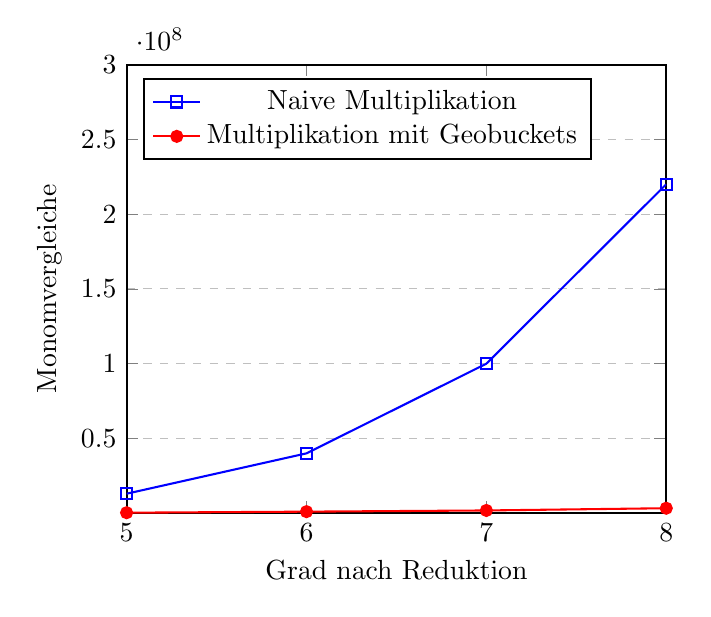
\begin{tikzpicture}
    \begin{axis}[
        xlabel={Grad nach Reduktion},
        ylabel={Monomvergleiche},
        xmin=5, xmax=8,
        ymin=100000, ymax=300000000,
        xtick={5,6,7,8},
        legend pos=north west,
        ymajorgrids=true,
        grid style=dashed,
    ]
    \addplot[
        color=blue,
        mark=square
        ]
        coordinates {
        (5, 13000000)(6, 40000000 )(7, 100000000)(8, 220000000)
        };
        \addlegendentry{Naive Multiplikation}
        
    \addplot[
        color=red,
        mark=*
        ]
        coordinates {
        (5, 300000)(6, 1000000 )(7, 1800000)(8, 3300000)
        };
        \addlegendentry{Multiplikation mit Geobuckets}
    
    \end{axis}
    \end{tikzpicture}
    \caption{Naive Multiplikation gegen Multiplikation mit Geobuckets}
    \label{fig:my_label}
\end{figure}



\newpage
%% ==============================
\section{Taylormodelle}
Taylormodelle bestehen in \verb+hotm+ aus einer List von nach der Ordnunng $\succ$ (siehe \ref{def:order}) sortierten Monomen. Für die Supportintervalle der Fehlersymbole wird eine statische Liste (\verb+static std::list+), für die Grenzwerte der Housekeeping-Methoden und den Index neuer Fehlersymbole jeweils statische Variablen angelegt.
\subsection{Housekeeping-Methoden}
Die Housekeeping-Methoden Splitting und Sweeping werden in \cite{DBLP:conf/macis/BrausseKM15} beschrieben und dienen der Kontrolle der Intervallkoeffizieten und deren Wachstum. Wann die Methoden angewandt werden, wird durch die manuell justierbaren Parameter \verb+MACRO_THRESHOLD+ für Splitting und \verb+MICRO_THRESHOLD+ für Cleaning festgelegt. Da für diese beiden Methoden Vergleiche reeller Zahlen nötig sind, um das Überschreiten eines Grenzwertes zu bestimmnen, werden die Zahlen mit Funktionen der \verb+iRRAM+ in rationale Approximationen zerlegt.

\paragraph{Cleaning}
Wie oben beschrieben, ergibt die Verwendung der \verb+iRRAM-REAL+s als Intervallgrenzen zweistufige Intervalle mit der Zahlen- und Intervallebene (siehe Abbildung \ref{fig:levels}). Mit fortlaufenden Rechnungen wächst die Breite der Intervalle auf Zahlenebene kontinuierlich und kann ohne weitere Methoden nur durch ein Erhöhen der verwendeten Präzision wieder verringer werden, beziehungsweise durch eine Iteration der \verb+iRRAM+. \textit{Cleaning} verlagert den Rechenfehler der Zahlenebene auf die Intervallebene und macht ihn damit auch für andere Housekeeping-Methoden sichtbar. Das Intervall $I=[m \pm r]$ mit $m=[c_m \pm \varepsilon_m]$ und $r = [c_r \pm \varepsilon_r]$ wird um $\varepsilon_m$ und $\varepsilon_r$ vergrößert, sodass das $I$ zwar wächst, jedoch dessen Endpunkte exakt sind:
\begin{align*}[[c_m \pm \varepsilon_m] \pm [c_r \pm \varepsilon_r]] &\rightsquigarrow [[c_m \pm 0] \pm [c_r + \varepsilon_m +\varepsilon_r  \pm 0]] \\
&= [\underbrace{c_m'}_{c_m + \varepsilon_m +\varepsilon_r} \pm c_r ]\end{align*}
    
    

\paragraph{Splitting}
Durch Cleaning, Sweeping oder eine Initialisierung der Taylormodelle mit einer gewissen Breite wachsen die Radii der Koeffizienten im Laufe einer Berechnung auch auf Intervallebene. Um die Überschätzung, die durch Intervallarithmetik entsteht zu kontrollieren, kann durch \textit{Splitting} ein Monom in zwei Monome mit Punktintervallen als Koeffizienten und einem neuen Fehlersymbol aufgeteilt werden:
\begin{align*}
[\tilde{c}_n \pm \varepsilon_n]\ \rightarrow [\tilde{c}_n \pm 0] + [\varepsilon_n \pm 0]\cdot  \lambda_n \hspace{0.5cm}, \lambda_n \in [0 \pm 1]
\end{align*}
Dadurch erhöht sich der Grad des Polynoms, jedoch verringert sich die Überschätzung durch Intervallarithmetik. Eine Alternative das Splitting zu realisieren ist, den Fehler statt wie in \cite{DBLP:conf/macis/BrausseKM15} im Koeffizienten des neuen Monoms, im neuen Fehlersymbol zu kodieren:
\begin{align*}
 [\tilde{c}_n \pm \varepsilon_n]\ \rightsquigarrow [\tilde{c}_n \pm 0] + [1 \pm 0]\cdot  \lambda_n \hspace{0.5cm}, \lambda_n \in [0 \pm \varepsilon_n]
\end{align*}
Dies hat den Vorteil, dass die Größe der Fehlersymbole beim Sweeping berücksichtigt werden kann.

\begin{algorithm}[H]
\label{algo:split}
\SetAlgoLined
\SetKwInOut{Input}{Eingabe}
\SetKwInOut{Output}{Ausgabe}
\Input{Taylormodell $T$: Liste von Monomen $m_i = c_i\cdot \lambda^i$ mit Koeffizienten $c_i = [\hat{c}_i \pm \varepsilon_i]$ und der Liste der Fehlersymbole $\lambda^i$, Grenzwert für Splitting $\delta_s $}
\Output{Taylormodell $T'$: Liste von Monomen mit Punktintervallkoeffizienten}
\DontPrintSemicolon
\ForAll{$i \in \{1,\dots, n\}$}{
    \uIf(\Comment*[f]{Die Intervallbreite überscheitet den Grenzwert}){$\varepsilon_i > \delta_s$ }{ 
        $s_{new} \gets [0 \pm \varepsilon_i]$ \Comment*{Führe neues Fehlersymbol ein} 
        $S \gets S \cup s_{new}$  \Comment*{\textit{Erweitere die Liste der Supportintervalle}} 
        $m_i' \gets [\hat{c_i}] \cdot \lambda^i$ \Comment*{Entferne den Radius von $m_i$}
        $m_i'' \gets [1] \cdot \lambda^i\lambda_{new}$ \Comment*{Erstelle ein neues Monom mit neuem Fehlersymbol}
        $T'\gets T' + m_i' + m_i''$
    } \Else{
        $T'\gets T' + m_i$
    }
}

\Return $T'$ \Comment*{Das neue Polynom hat maximal $2n+1$ Monome }
 \caption{Algorithmus für Splitting}
\end{algorithm}




\paragraph{Sweeping}
Cleaning und Splitting sorgen dafür, dass die Intervallbreite der Koeffizienten klein bleibt, jedoch erhöht sich der Grad der Polynome, was zum Beispiel bei der Multiplikation von Taylormodellen zu Ineffizienz durch die exponentiell wachsende Anzahl an Monomen führt. Um diesem Effekt entgegenzuwirken, kann mit \textit{Sweeping} ein Fehlersymbol durch sein Supportintervall ersetzt werden:
\begin{align*}
 c_n \lambda_i^k \rightsquigarrow c_n s_i \lambda_i^{k-1}
\end{align*}
Hierbei ist zu beachten, dass das $n$-fache Sweepen eines Fehlersymbols, welches die 0 enthält, mit $n$ gerade eine geringere Breite in den Koeffizienten einführt, als $n$ ungerade (siehe oben \ref{par:potenzfunktion}). Daraus ergeben sich zwei Sweeping-\textit{Strategien}.

\subparagraph{square\_only}
Die Sweeping-Strategie \verb+square_only+ beschränkt das Sweeping auf gerade Potenzen. So wird die angestrebte Reduktion des Grades eines Monoms nur erreicht, wenn alle Variablen einen geraden Exponenten haben.


\begin{algorithm}[H]
\label{algo:split}
\SetAlgoLined
\SetKwInOut{Input}{Eingabe}
\SetKwInOut{Output}{Ausgabe}
\Input{Taylormodell $T$: Liste von Monomen $m_i = c_i\cdot \lambda^i$ mit Koeffizienten $c_i = [\hat{c}_i \pm \varepsilon_i]$ und der Liste der Fehlersymbole $\lambda^i$, Zielgrad $\gamma$}
\Output{Taylormodell $T'$: Liste von Monomen mit Punktintervallkoeffizienten}
\DontPrintSemicolon
\ForAll{$i \in \{0,\dots, n\}$}{
    $o \gets grad(m_i)$\\
    \uIf{$o \leq \gamma$}{
        $T' \gets T' + m_i$
    }\Else{
        $c_i' \gets c_i$ \\
        $\lambda^{i'}\gets \{\lambda^l_j | \lambda_j^l \in \lambda^i \land |s_j| < |s_{j+1}| \} $\\
        $r\gets o - \gamma$\\
        \ForAll{$\lambda^l_j \in \lambda^{i'}$}{
            $p \gets min(l, r)$\\
            \lIf{$p > 1$ \textbf{and} $2 \nmid p$}{$p \gets p-1$}
            $r \gets r - p$ \\
            $c_i' \gets c_i' \cdot \lambda_j^p$\\
            $l \gets l-p$\\
            \lIf{$r < 2$}{\textbf{break}}
        }
        $\lambda^{i'}\gets \{\lambda^l_j | \lambda_j^l \in \lambda^{i'} \land \lambda_j \succ \lambda_{j+1} \} $\\
        $T' \gets T' + c_i' \cdot \lambda^{i'}$
    }
}

\Return $T'$ 
 \caption{Algorithmus für Sweeping mit square\_only}
\end{algorithm}



\subparagraph{square\_first}
Mit \verb+square_first+ wird der angestrebte Grad erreicht, indem zunächst möglichst viele Fehlersymbole gerade gesweept werden. Falls dadurch jedoch nicht die gesamte Reduktion möglich ist, wird der Rest ungerade gesweept.

Der Aufruf der Methode erhält in \verb+hotm+ drei Parameter; das zu reduziere Taylormodell, den Grad, auf das Taylormodell durch Sweeping reduziert werden soll und die Strategie:

 \begin{lstlisting}[language=C++, caption=Beispielaufruf der Sweeping-Routine,captionpos=b,xleftmargin=15pt]
tmsimple x;
x = sweep_to(x, 2, SQUARE_ONLY);
\end{lstlisting}



\subsection{Darstellung der Taylormodelle}
Die grafischen Darstellungen der Taylormodelle in dieser Arbeit wurden mit \verb+gnuplot+ \cite{gnuplot} erstellt und zeigen je eine Übermenge des tatsächlichen Taylormodells. Eine Darstellung eines Taylormodells entsteht, indem für jedes der $k$ Fehlersymbol aus $\lambda=(\lambda_1, \dots, \lambda_k)$ ein Wert festgelegt und dann das Taylormodell evaluiert wird. Um eine Übermenge zu zeichnen muss der gesamte Wertebereich eines jeden Fehlersymbols abgedeckt werden. In \verb+hotm+ geschieht das, indem für eine gegebene \textit{Auflösung} $a \in \mathbb{N}$ die Supportintervalle $S=(s_1, \cdots s_k)$ in jeweils $a$ Intervalle geteilt und für jede Kombination mit eingesetzten Werten ein von den anderen unabhängiges Rechteck gezeichnet wird. So ergeben sich für Taylormodelle mit $k$ Variablen $a^k$ Rechtecke. Eine solche Darstellung wird in \cite{DBLP:conf/macis/BrausseKM15} als $image(T) \subseteq \mathbb{R}^d$ definiert. Die hier verwendete Darstellung wird um die verwendete Auflösung erweitert: $image_{acc}(T,a)$.

\Abbildungps{tbh}{.9}{img/accuracy.pdf}{fig:acc}{H\e non-Abbildung: Abbildung mit verschiedenen Auflösungen}{Jede Zeile zeigt eine einfache Abbildung der Rechtecke durch die H\e non-Abbildung mit $a=1.4$ und $b=0.3$ mit verschiedenen Auflösungen für die Darstellung. (a): 4 Rechtecke; (b): 100 Rechtecke, (c): 10000 Rechtecke. Das Tetragon stellt die Fangzone für die verwendeten Parameter dar. }

Seien $T_1$ und $T_2$ Taylormodelle mit $k=2$ Variablen, die eine zweidimensionale Fläche aufspannen, bei denen die initialen Fehlersymbole erhalten bleiben und keine neuen Fehlersymbole eigeführt werden, so kann durch die Abhängigkeitsinformation der Fehlersymbole Ursprung und Abbild der einzelnen Regionen dieser Fläche farblich induziert werden. Abbildung \ref{fig:acc} zeigt eine Iteration der H\e non-Abbildung eines Rechtecks mit verschiedenen Auflösungen. Es ist gut zu erkennen, dass die gröbere Auflösungen, die feinere überdeckt und $image_{acc}(T_1,100)\times image_{acc}(T_2,100) \subseteq image_{acc}(T_1,10)\times image_{acc}(T_2,10) \subseteq image_{acc}(T_1,2)\times image_{acc}(T_2,2) $ gilt. Durch die Einfärbung der Rechtecke können verschiedene Effekte beobachtet werden:
\begin{enumerate}
 \item Die Rechtecke überlagern sich im Abbild, obwohl sie sich im Ursprung nicht überschneiden und die H\e non-Abbildung an sich eindeutig invertierbar ist. Grund hierfür ist die entstehende Überschätzung durch Intervallarithmetik, die besonders bei Multiplikation, beziehungsweise Quadrierung der Intervalle zum Tragen kommt.
 \item Das in den Grafiken eingezeichnete Tetragon stellt die Fangzone $R$ für die hier verwendeten Parameter $a=1.4$ und $b=0.3$ dar. Mit Hilfe der Einfärbung ist erkennbar, wie Regionen außerhalb von $R$ wiederum außerhalb abgebildet werden, während innerhalb liegende diese nach der Abbildung nicht verlassen.
\end{enumerate}










%%% Local Variables: 
%%% mode: latex
%%% TeX-master: "thesis"
%%% End: 
